
\paragraph{DELETE /:lang/user/:userId}
\begin{itemize}
\item \textbf{Successo} \\
	\textbf{Descrizione}:

\begin{figure}[ht]
	\centering
	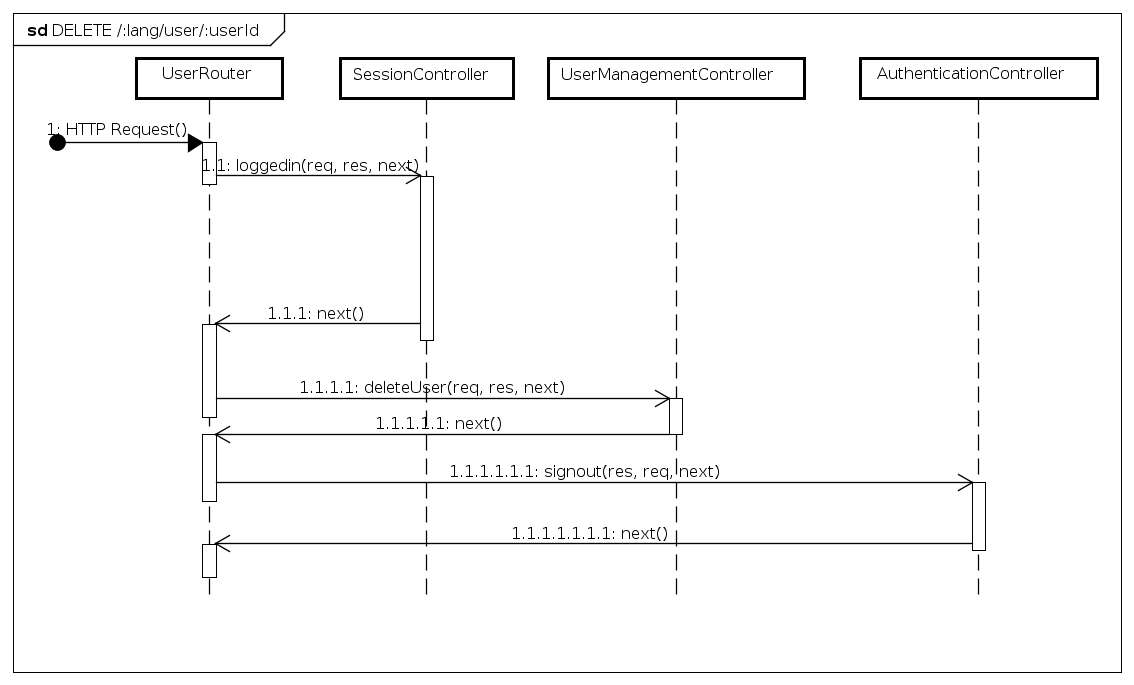
\includegraphics[scale=0.45]{UML/DiagrammiDiSequenza/Back-end/DELETE __lang_user__userId_success.png}
	\caption{DELETE /:lang/user/:userId}
\end{figure}
\FloatBarrier

\item \textbf{Fallimento} \\
	\textbf{Descrizione}:

\begin{figure}[ht]
	\centering
	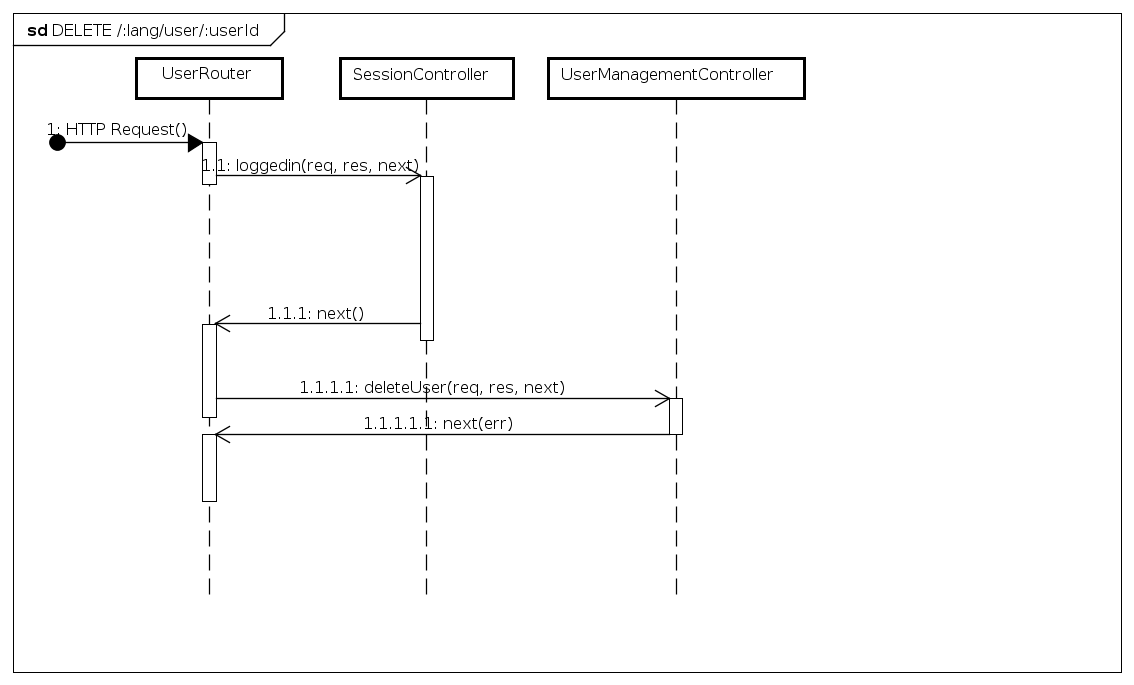
\includegraphics[scale=0.45]{UML/DiagrammiDiSequenza/Back-end/DELETE __lang_user__userId_failure.png}
	\caption{DELETE /:lang/user/:userId}
\end{figure}
\FloatBarrier


\end{itemize}

\paragraph{GET /:lang/user/:userId}
\begin{itemize}
\item \textbf{Successo}
% descrizione diagramma e UML
\item \textbf{Fallimento}
% descrizione diagramma e UML
\end{itemize}

\paragraph{PUT /:lang/user/:userId}
\begin{itemize}
\item \textbf{Successo}
% descrizione diagramma e UML
\item \textbf{Fallimento}
% descrizione diagramma e UML
\end{itemize}

\paragraph{PUT /:lang/user/:userId/privacy}
\begin{itemize}
\item \textbf{Successo}
% descrizione diagramma e UML
\item \textbf{Fallimento}
% descrizione diagramma e UML
\end{itemize}


\paragraph{GET /:lang/user/:userId/statistics}
\begin{itemize}
\item \textbf{Successo}
% descrizione diagramma e UML
\item \textbf{Fallimento}
% descrizione diagramma e UML
\end{itemize}

\paragraph{GET /:lang/user/:userId/statistics/summary/}
\begin{itemize}
\item \textbf{Successo}
% descrizione diagramma e UML
\item \textbf{Fallimento}
% descrizione diagramma e UML
\end{itemize}


\paragraph{GET /:lang/user/:userId/statistics/summary/:summaryId}
\begin{itemize}
\item \textbf{Successo}
% descrizione diagramma e UML
\item \textbf{Fallimento}
% descrizione diagramma e UML
\end{itemize}



